\documentclass[a4paper,11pt]{article}

\usepackage{préambule}

\addtolength{\oddsidemargin}{-1.5cm}
\addtolength{\evensidemargin}{-1.5cm}
\addtolength{\textwidth}{2.5cm}
\addtolength{\textheight}{0.5cm}

\title{Activité : Symétrie axiale}
\date{}
\author{}

% Ceux jeu est fortement tiré de la brochure A.P.M.E.P. n∘69 - 2005.
\begin{document}

\begin{center}
	\LARGE
	Activité : Symétrie axiale
\end{center}

\vspace{1em}

\begin{greybox}[frametitle={⚠ Avant de commencer ⚠}]
	\begin{center}
		{\Large\textbf{Commence par découper les pièces qui t'ont été données \uline{sur l'autre feuille}.}}
	\end{center}
\end{greybox}


\begin{exercice}\ \\
	Quelles sont les pièces qui ont un ou plusieurs axes de symétrie ? \\
	Dessine ces pièces sur la grille ci-dessous, et trace en pointillé leurs axes de symétrie.\\[1em]
	\begin{tikzpicture}[scale=1.71]
		\draw[step=1.0,gray,thin] (0,0) grid (11,3);
	\end{tikzpicture}
\end{exercice}

\begin{exercice}\ \\
	\parbox[b]{0.8\textwidth}{Tu as remarqué que toutes les pièces vont par paires. On peut les disposer de manière symétrique, comme ceci :
	}
	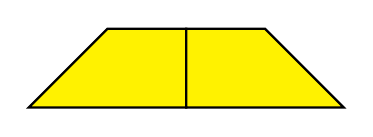
\begin{tikzpicture}
		\draw[black,fill=yellow,thick] (0,0) -- ++(2,0) -- ++(0,1) -- ++(-1,0) -- cycle;
		\draw[black,fill=yellow,thick] (2,0) -- ++(0,1) -- ++(1,0) -- ++(1,-1) -- cycle;
	\end{tikzpicture}

	Dessine chaque paire de pièce sur la grille ci-dessous :\\[1em]
	\begin{tikzpicture}[scale=1.71]
		\draw[step=1.0,gray,thin] (0,0) grid (11,7);
	\end{tikzpicture}
\end{exercice}

\begin{exercice}\ \\
	\begin{minipage}{0.55\textwidth}
		On peut utiliser 6 pièces pour faire un rectangle comme ci-contre. La figure obtenue a un axe de symétrie.
	\end{minipage}
	\begin{minipage}{0.05\textwidth}
		\hspace{0.05\textwidth}
	\end{minipage}
	\begin{minipage}{0.4\textwidth}
		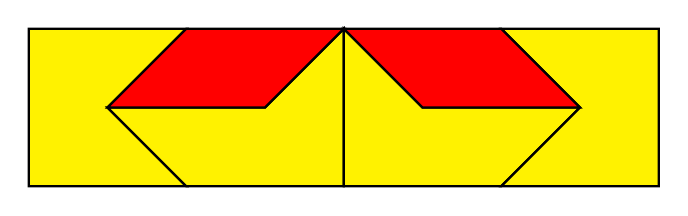
\begin{tikzpicture}
			\draw[black,fill=yellow,thick] (0,0) -- ++(2,0) -- ++(-1,1) -- ++(1,1) -- ++(-2,0) -- cycle;
			\draw[black,fill=yellow,thick] (2,0) -- ++(2,0) -- ++(0,2) -- ++(-1,-1) -- ++(-2,0) -- cycle;
			\draw[black,fill=red,thick] (1,1) -- ++(2,0) -- ++(1,1) -- ++(-2,0) -- cycle;

			\draw[black,fill=yellow,thick] (4,0) -- ++(2,0) -- ++(1,1) -- ++(-2,0) -- ++(-1,1) -- cycle;
			\draw[black,fill=yellow,thick] (6,0) -- ++(2,0) -- ++(0,2) -- ++(-2,0) -- ++(1,-1) -- cycle;
			\draw[black,fill=red,thick] (4,2) -- ++(1,-1) -- ++(2,0) -- ++(-1,1) -- cycle;
		\end{tikzpicture}
	\end{minipage}

	De manière similaire, utilise les pièces indiquées pour faire un rectangle avec un axe de symétrie : \\
	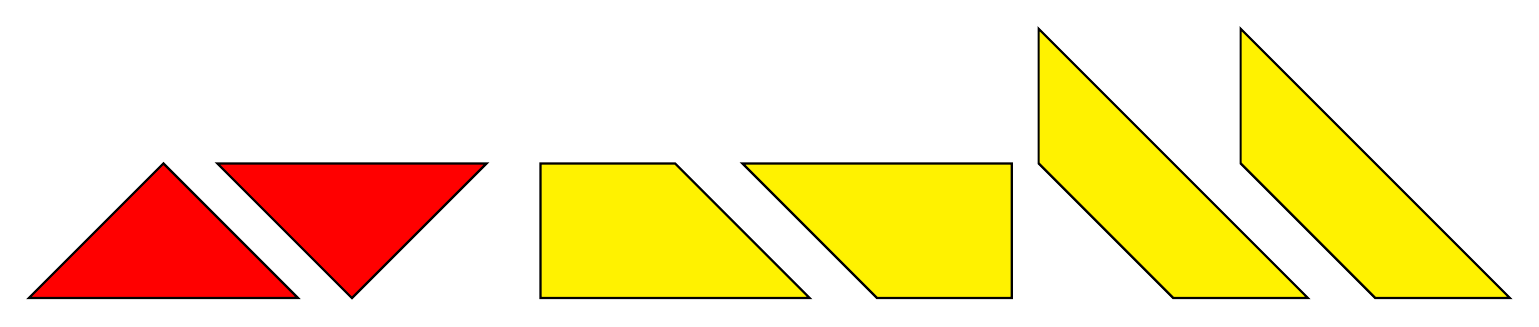
\begin{tikzpicture}[scale=1.71]
		\draw[black,fill=red,thick] (0,0) -- ++(2,0) -- ++(-1,1) -- cycle;
		\draw[black,fill=red,thick] (1.4,1) -- ++(2,0) -- ++(-1,-1) -- cycle;

		\draw[black,fill=yellow,thick] (3.8,0) -- ++(2,0) -- ++(-1,1) -- ++(-1,0) -- cycle;
		\draw[black,fill=yellow,thick] (6.3,0) -- ++(1,0) -- ++(0,1) -- ++(-2,0) -- cycle;

		\draw[black,fill=yellow,thick] (8.5,0) -- ++(1,0) -- ++(-2,2) -- ++(0,-1) -- cycle;
		\draw[black,fill=yellow,thick] (10,0) -- ++(1,0) -- ++(-2,2) -- ++(0,-1) -- cycle;
	\end{tikzpicture} \\[1em]
	\begin{tikzpicture}[scale=1.71]
		\draw[step=1.0,gray,thin] (0,0) grid (11,5);
	\end{tikzpicture}
\end{exercice}

\begin{exercice}\squared{\large\textbf{⚠ Demande une grille au professeur. ⚠}}

	\begin{minipage}{0.7\textwidth}
		\begin{enumerate}
			\item Observe le dessin ci-contre. C'est une figure qui admet un axe de symétrie. En utilisant \textbf{toutes} les pièces du jeu, reproduit cette figure. Note ta solution sur le premier carré ci-dessous.
			\item Réorganise tes pièces pour avoir un motif symétrique par rapport à un axe horizontal, vertical ou diagonal.

			      Trouve 3 solutions différentes, et dessine chacune d'entre elles ci-dessous.
		\end{enumerate}
	\end{minipage}
	\begin{minipage}{0.05\textwidth}\hspace{\textwidth}\end{minipage}
	\begin{minipage}{0.25\textwidth}
		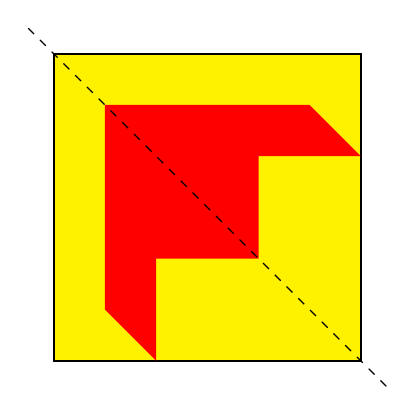
\begin{tikzpicture}[scale=0.65]
			\draw[black,fill=yellow,thick] (0,0) rectangle (6,6);
			\fill[red] (2,0) -- ++(0,2) -- ++(2,0) -- ++(0,2) -- ++(2,0) -- ++(-1,1) -- ++(-4,0) -- ++(0,-4) -- cycle;
			\draw[dashed] (-0.5,6.5) -- (6.5,-0.5);
		\end{tikzpicture}
	\end{minipage}

	\vspace{1em}

	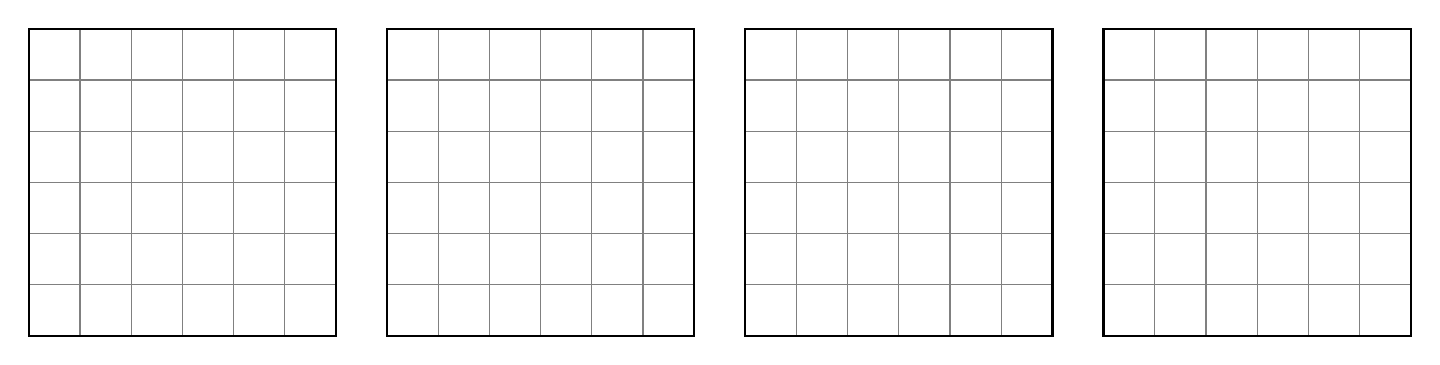
\begin{tikzpicture}[scale=0.65]
		\draw[step=1.0,gray,thin] (0,0) grid ++(6,6);
		\draw[black,thick] (0,0) rectangle ++(6,6);

		\draw[step=1.0,gray,thin] (7,0) grid ++(6,6);
		\draw[black,thick] (7,0) rectangle ++(6,6);

		\draw[step=1.0,gray,thin] (14,0) grid ++(6,6);
		\draw[black,thick] (14,0) rectangle ++(6,6);

		\draw[step=1.0,gray,thin] (21,0) grid ++(6,6);
		\draw[black,thick] (21,0) rectangle ++(6,6);
	\end{tikzpicture}
\end{exercice}

\end{document}